\documentclass[11pt,a4paper,titlepage]{article}
\usepackage{graphicx}
\usepackage[margin=1in]{geometry}
%\usepackage{titling}
\usepackage[hidelinks]{hyperref}


\usepackage{epstopdf}

\DeclareGraphicsExtensions{.png}
\DeclareGraphicsExtensions{.jpg}
%\DeclareGraphicsExtensions{.eps}

\begin{document}
\begin{titlepage}
	\begin{center}
		
		\begin{figure}[t]
			\centering
			
\includegraphics[width=350px]{UP_Logo.png}
		\end{figure}		
	
	
	\begin{flushright} 
		
		\textbf{\LARGE COS 301 Main Project}
		\newline \newline \newline
		\textbf{\LARGE Requirements and Design Specifications}
		\newline \newline \newline
 		\textbf{\LARGE ThinkTech}
		\newline \newline \newline
	\end{flushright}
		
		\vspace{1 cm}
		
		\LARGE{\textbf{Group Members: }}
		
		%\begin{minipage}{0.4\textwidth}

		\begin{flushright} \large
			Lelethu Zazaza 13028023\newline
			Goodness Adegbenro 13046412\newline
		\end{flushright}
		%\end{minipage}
		
	
		
		\textbf{Git repository link:\\}
		 \url{ https://github.com/COS301-ThinkTech}
		
		\vfill
		
		{\LARGE Version 0.1}
		\\
		{\large \today}		
		
		
	\end{center}
\end{titlepage}


\tableofcontents
\pagebreak

\section{Vision and scope}
\subsection{Project background}
\subsection{Project vision}

This project sets out to create an application for the planning and simulation of flowcharts, which
can be used in an education setting for an introductory program logic course. The objective is to
develop an application that can feasibly be used in such a practical setting. The application must be
visual in nature, due to the visual nature of flowcharts. The application must facilitate exploration
and experimentation, while providing clear feedback to the user as to how the program executes.

\subsection{Project scope}

The project consists of the following two components:

\begin{itemize}
\item A planning canvas, in which a flowchart can be built using an intuitive drag-and-drop editor.
Flowchart components will be selected and dropped into the canvas, and connected into
complete flowcharts. The system will also have to do error checking on the constructed
flowcharts, so that (for example) multiple entry points into a program or certain flowchart
components are not allowed.
\item An execution system, in which a flowchart can be run from start to finish. The system
should allow for one-click execution of the entire program, as well as step-by-step
execution. At all stages during execution, the currently executing component should be
highlighted, as well as the connection path being followed. The program's execution should
be very visually apparent and appealing. The output of the flowchart's execution should also
be apparent.
\end{itemize}

The following components are specifically excluded from the scope of the project:

\begin{itemize}
\item No executable program code generation will be required for this project.
\item No complex design elements (such as user-defined component assemblies) are required.
Only the basic components of standard flowcharts are necessary.\\

\end{itemize}

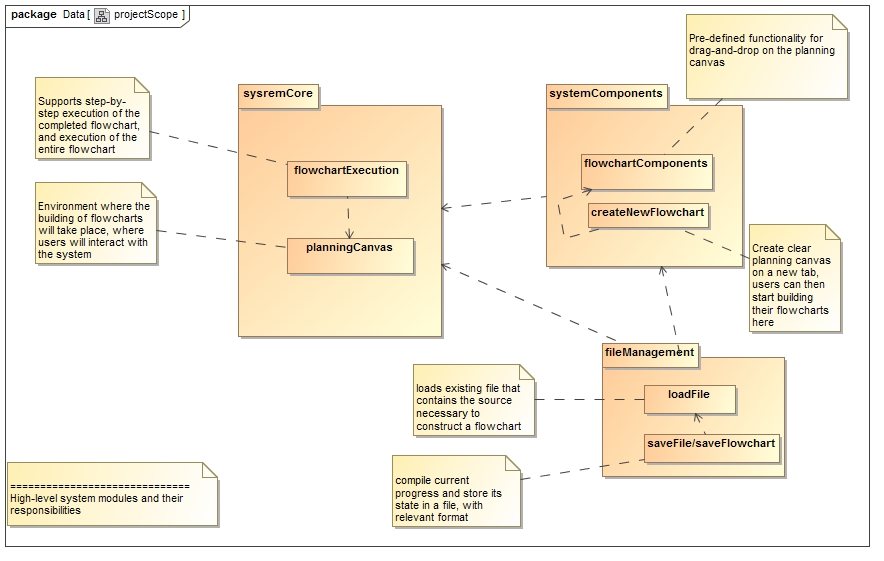
\includegraphics[width=500px]{projectScope.jpg}
\centerline{High level system modules and their responsibilities.}
% Include auxillary files here:  \input{file} 


\newpage	
\section{Use case prioritization}
\subsection{Critical}
\begin{itemize}
  \item createNewFlowchart
\end{itemize}
\subsection{Important}
\begin{itemize}
  \item addFlowchartComponent
  \item editFlowchartComponent
  \item saveFlowchart
  \item loadFlowchart
  \item deleteFlowchartComponent
  \item executeFlowchart
\end{itemize}

\newpage
\section{Use cases}
	
\subsection{deleteFlowchartProject}
The deleteFlowchartProject use case serves the purpose of removing a flowchart project.

\subsubsection{Use case diagram}
%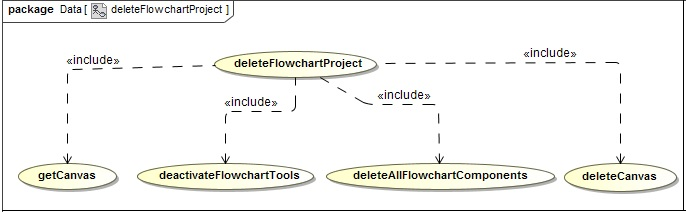
\includegraphics[width=500px]{deleteFlowchartProjectUseCase.jpg}

\subsubsection{Activity diagram}
%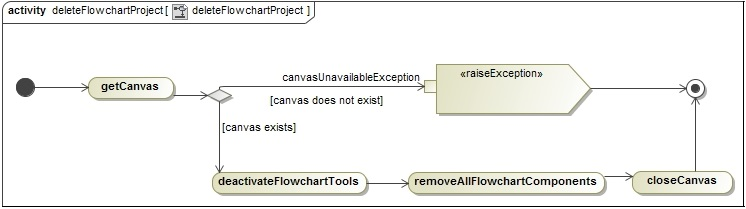
\includegraphics[width=500px]{deleteFlowchartProject.jpg}

\subsection{editFlowchartComponent}
The editFlowchartComponent use case provides functionality for the user to edit each component of the flowchart on a canvas.\newline\newline
\textbf{Pre Condition:} Component must have been added\newline\newline
\textbf{Post Condition:} Component has been edited

\subsubsection{Use case diagram}
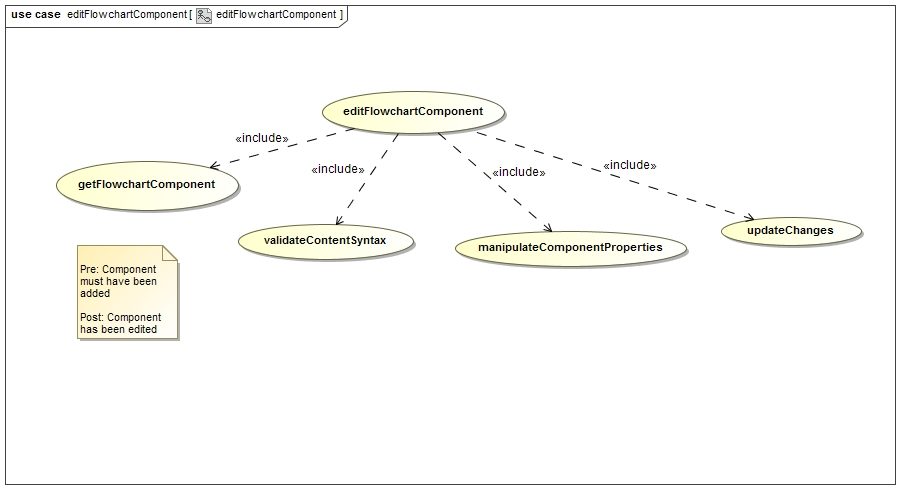
\includegraphics[width=500px]{editFlowchartComponentUseCase.jpg}

\subsubsection{Activity diagram}
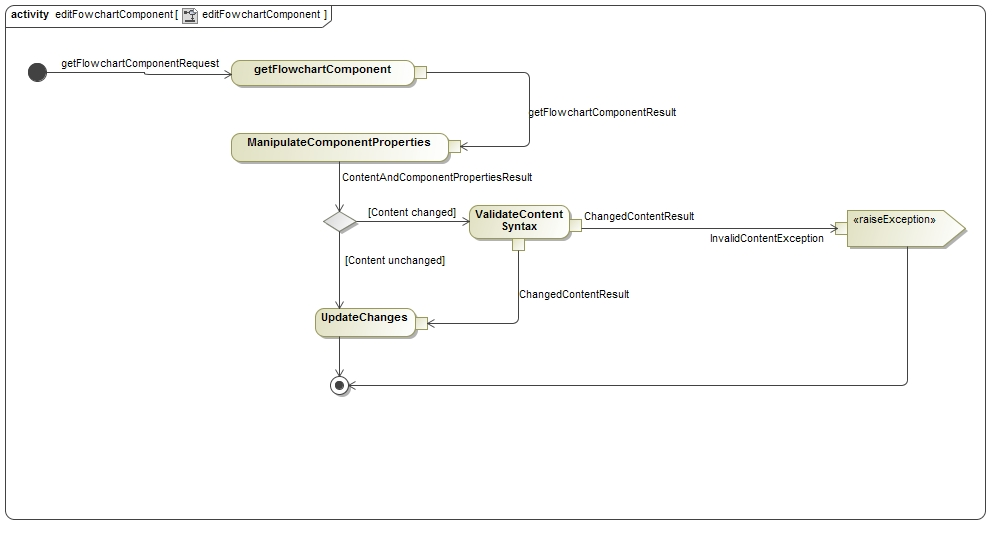
\includegraphics[width=500px]{editFowchartComponent.jpg}

\subsection{saveFlowchart}
The saveFlowchart use case provides functionality for the user to save a flowchart.\newline\newline
\textbf{Pre Condition:} Canvas is open\newline\newline
\textbf{Post Condition:} Flowchart has been saved to file

\subsubsection{Use case diagram}
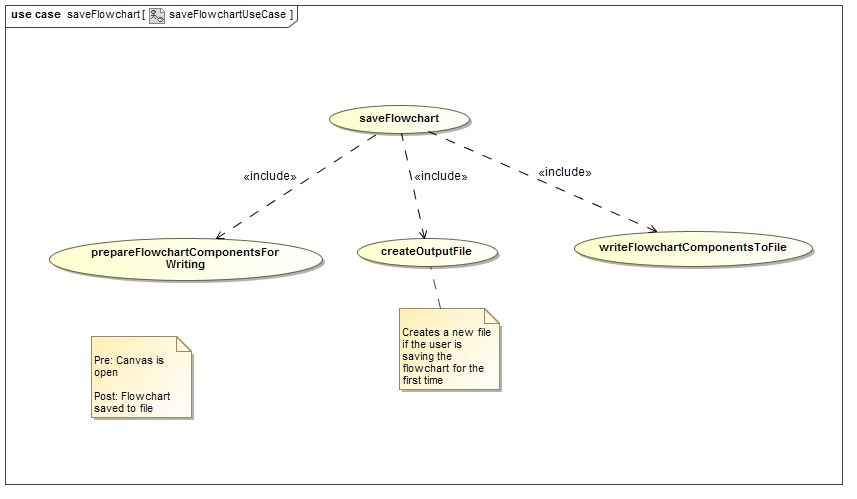
\includegraphics[width=500px]{saveFlowchartUseCase.jpg}

\subsubsection{Activity diagram}
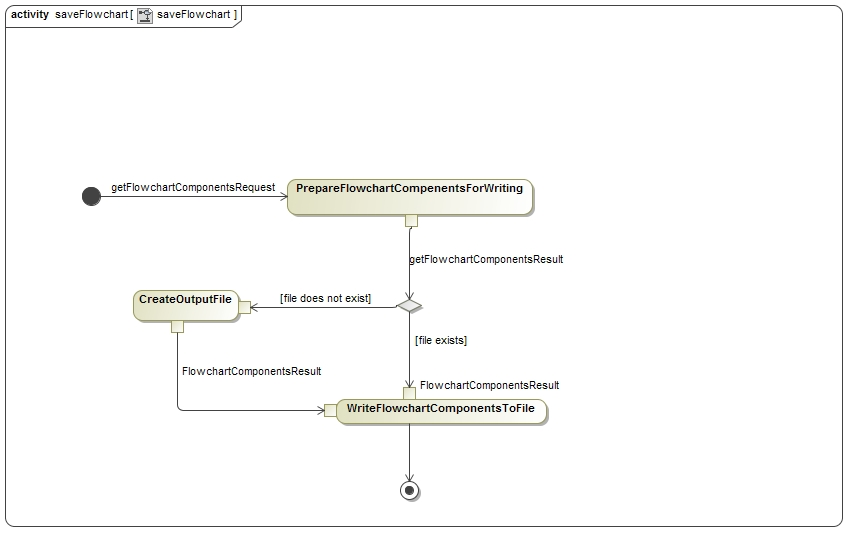
\includegraphics[width=500px]{saveFlowchart.jpg}

\subsection{loadFlowchart}
loadFlowchart: users load flowcharts from existing files. The file is editable, can be modified by the user.\newline\newline
\textbf{Pre Condition:} file with correct extension already exists.\newline
\textbf{Post Condition:} open the file and make it editable in the canvas element.

\subsubsection{Use case diagram}
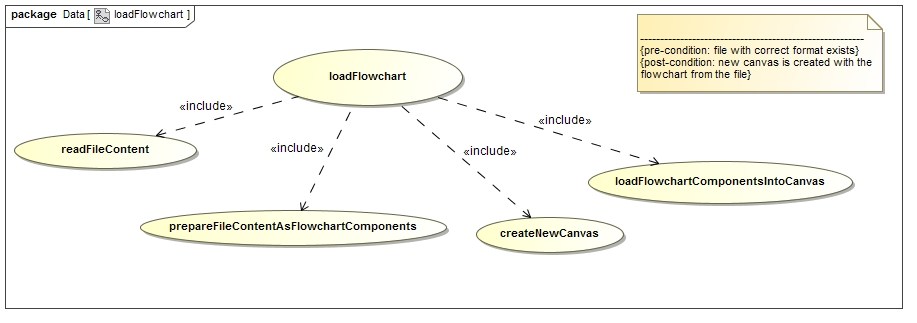
\includegraphics[width=500px]{loadFlowchart_use_case_diagram.jpg}

\subsubsection{Activity diagram}
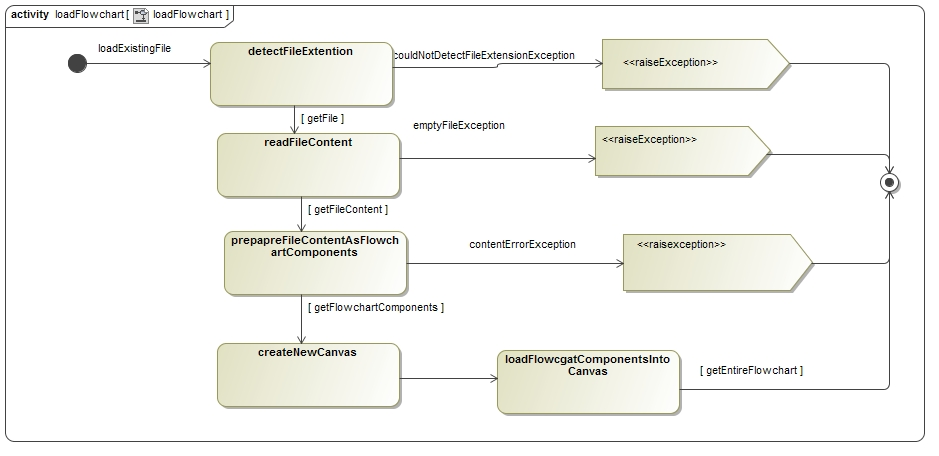
\includegraphics[width=500px]{loadFlowchart_activity_diagram.jpg}

\subsubsection{Domain mode}
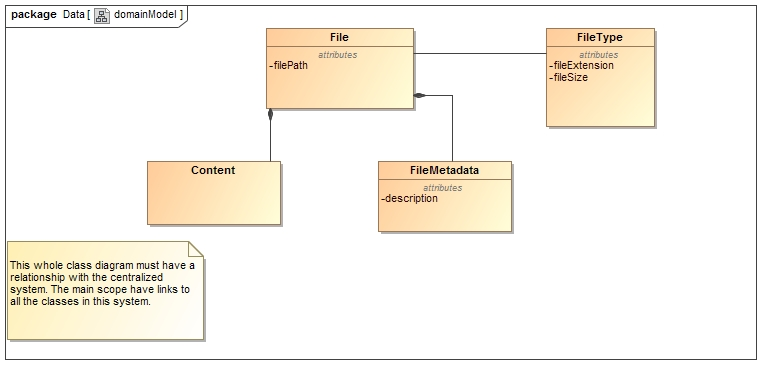
\includegraphics[width=500px]{loadFlowchart_domain_model.jpg}

\subsection{deleteFlowchartComponent}
The deleteFlowchartComponent use case enables the functionality to delete individual components from the canvas.
\newline\newline
\textbf{Pre Condition:} The canvas has to be available. Component exists in the canvas space and is in the components list.
\newline\newline
\textbf{Post Condition:} The canvas is clear of any components that were selected for removal.

\subsubsection{Use case diagram}
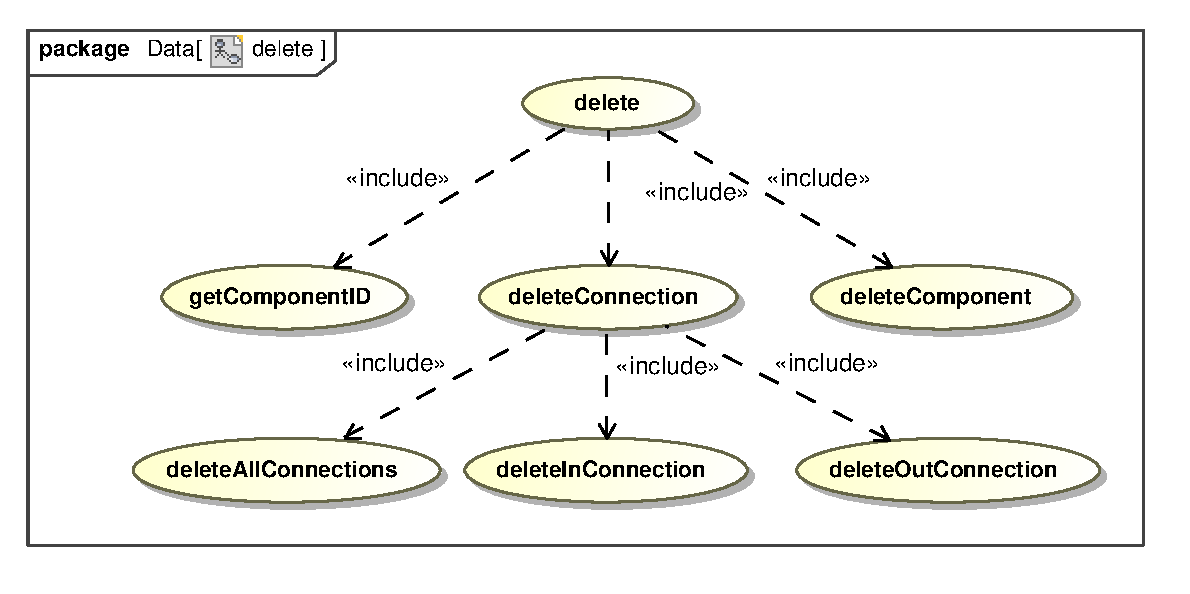
\includegraphics[width=500px]{delete.eps}

\subsubsection{Activity diagram}
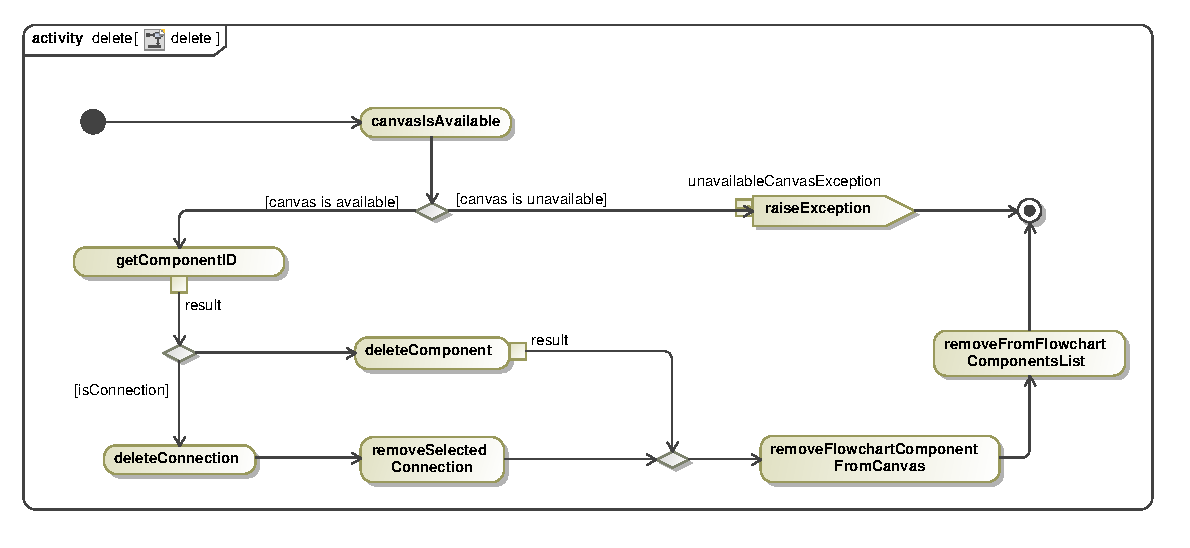
\includegraphics[width=500px]{deleteAct.eps}

\subsection{executeFlowchart}
The executeFlowchart use case enables the functionality to execute the flowchart step-by-step or from start-to-end.
\newline\newline
\textbf{Pre Condition:} Canvas has to be available.
\newline\newline
\textbf{Post Condition:} Flowchart will return feedback of any errors, warnings or successful execution along with the results of any calculations.

\subsubsection{Use case diagram}
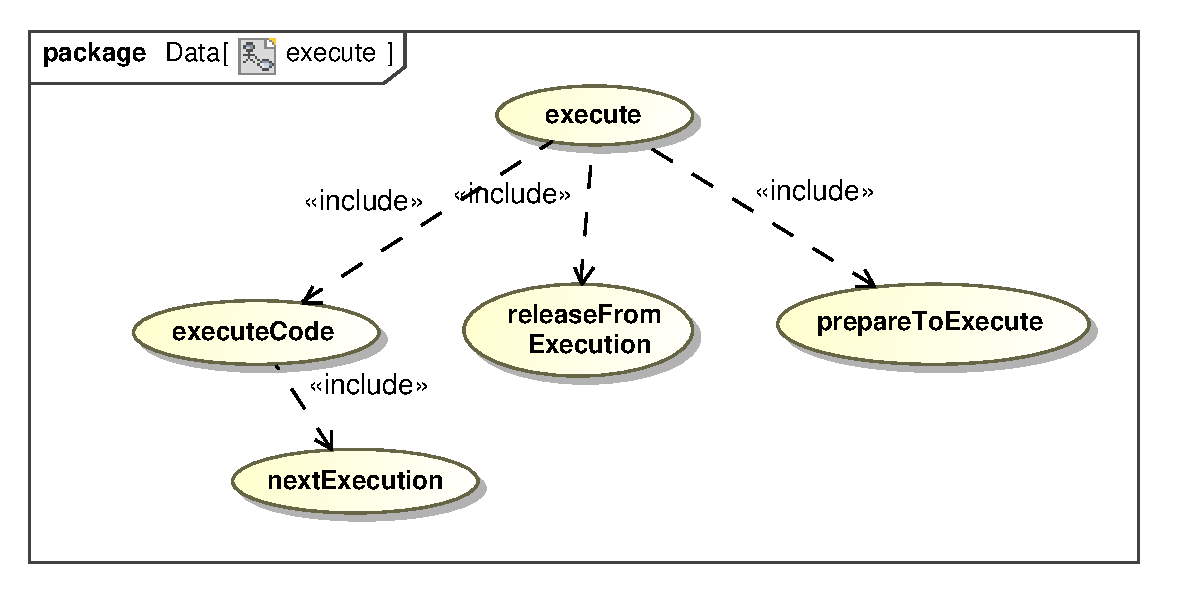
\includegraphics[width=500px]{execute.eps}

\subsubsection{Activity diagram}
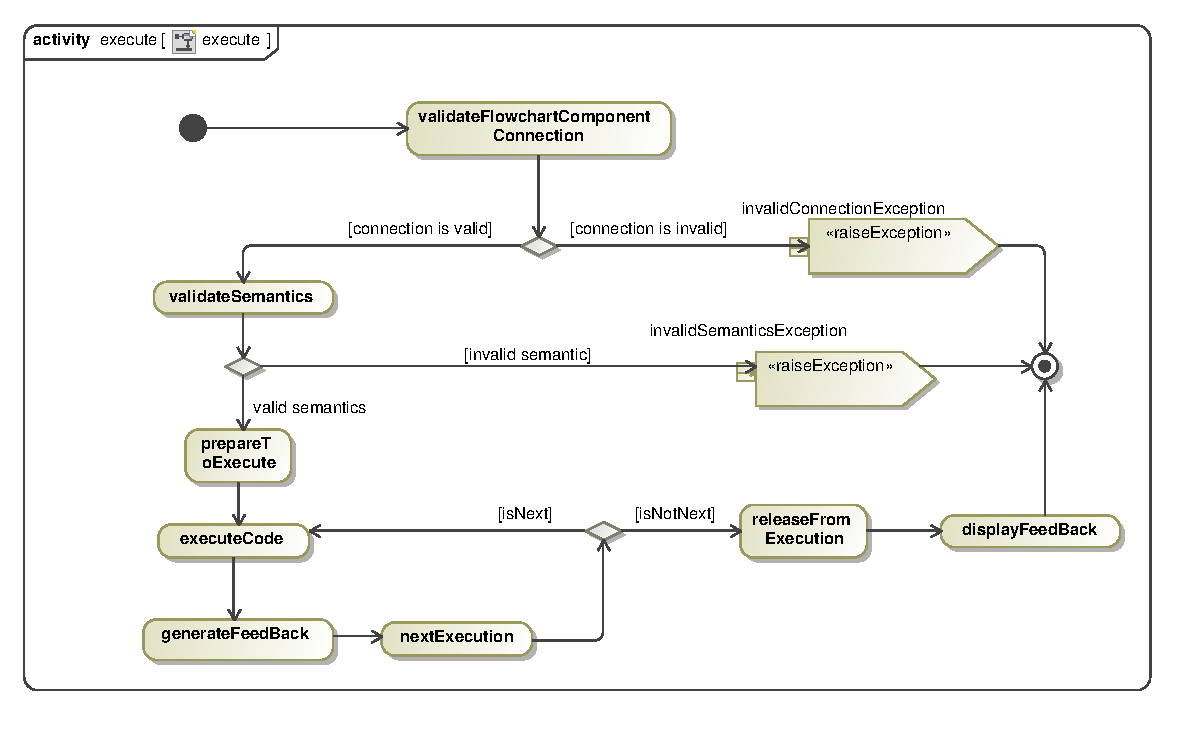
\includegraphics[width=500px]{executeAct.eps}

\end{document}
